\chapter{MODEL EVALUATION}
\label{ch:evaluation}
This chapter evaluates how well the trained models perform by testing them on a designated dataset. The models are assessed using the best hyper-parameters from the previous chapter. Metrics like precision, recall, and F1-score are used, along with visual tools like confusion matrices. The results show how well each model handles new data.

\section{Methodology}
The train set constitutes 30\% of the total data set. This corresponds to 2216 images. I used a stratified split, which guarantees that the proportions of number of images in each class is maintained in the test set. The confusion matrix and other metrics presented in this section were made with the model predictions of this test set. At this point the model is already using the most adequate hyper-parameters found in the previous hyper-parameter tuning phase. 

\section{Simple Neural Network Evaluation}
In Fig. 5.1 there is a heat map representation of the obtained confusion matrix for the simple neural network model. It can be observed that the model has problems predicting most of the classes. Instead, it seemed to favor few breeds, choosing them most of the time. Other metrics were also calculated and are summarized in the table 5.1.
   \begin{figure}[H]
    \centering
    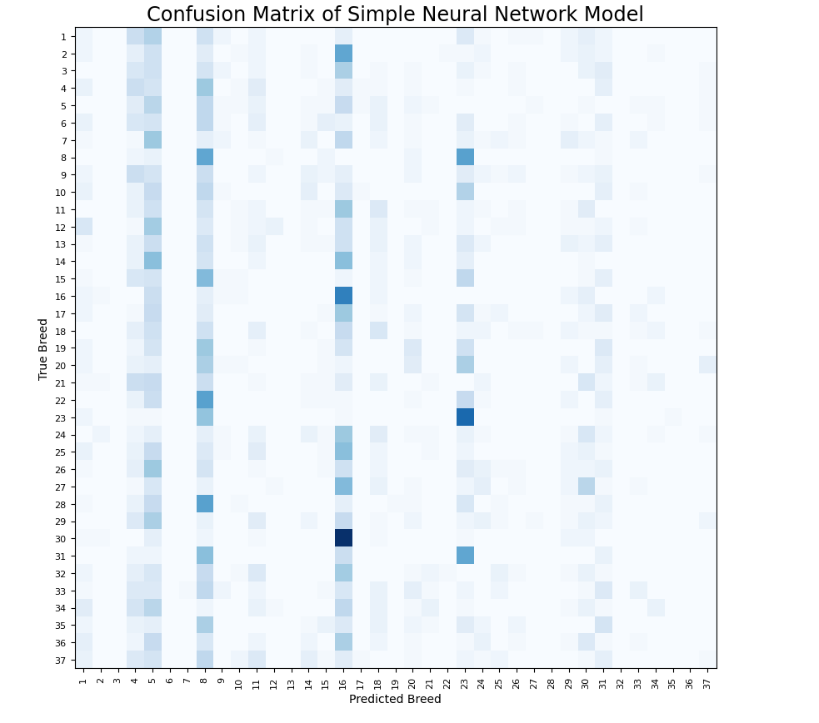
\includegraphics[width=0.7\textwidth]{figures/ssn_cm.png}
    \caption{Confusion matrix heat map for simple neural network}
    \label{fig:example_images}
\end{figure}
\begin{table}[H]
    \centering
    \caption{Metric Evaluation for Simple Model}
    \begin{tabular}{|c|c|c|c|}
        \hline
        Metric & Precision & Recall & F1-score \\ 
        \hline
        Macro Average & 0.05 & 0.07 & 0.06 \\ 
        \hline
        Weighted Average & 0.06 & 0.066 & 0.06 \\ 
        \hline
    \end{tabular}
    \label{tab:simple_model_metrics}
\end{table}


\section{Complex Neural Network Evaluation} 
Fig. 5.2 is a heat map representation of the obtained confusion matrix. It can be seen that the model had some trouble breed no. 27 (i.e ragdoll cat). It often predicted the breed birman instead of it. When looking at the images shown in Fig 5.3, it can be seen why this happens, since they look really similar to one another.Other metrics were also calculated and are summarized in
 the table 5.2.
    \begin{figure}[H]
    \centering
    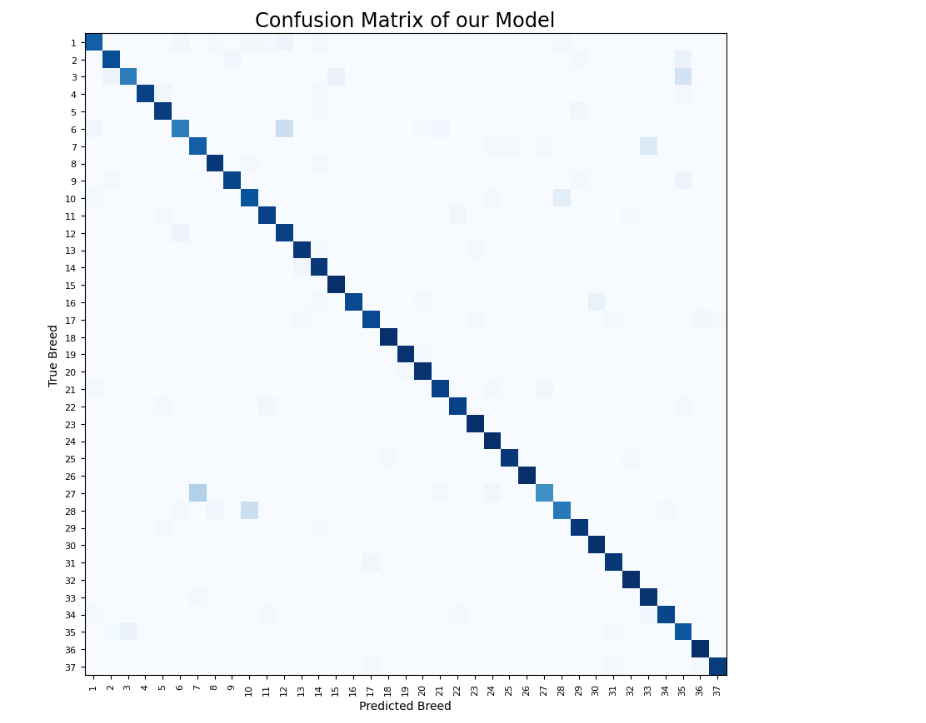
\includegraphics[width=0.7\textwidth]{figures/confusion matrix.png}
    \caption{Confusion matrix heat map for complex neural network}
    \label{fig:example_images}
\end{figure}
    \begin{figure}[H]
    \centering
    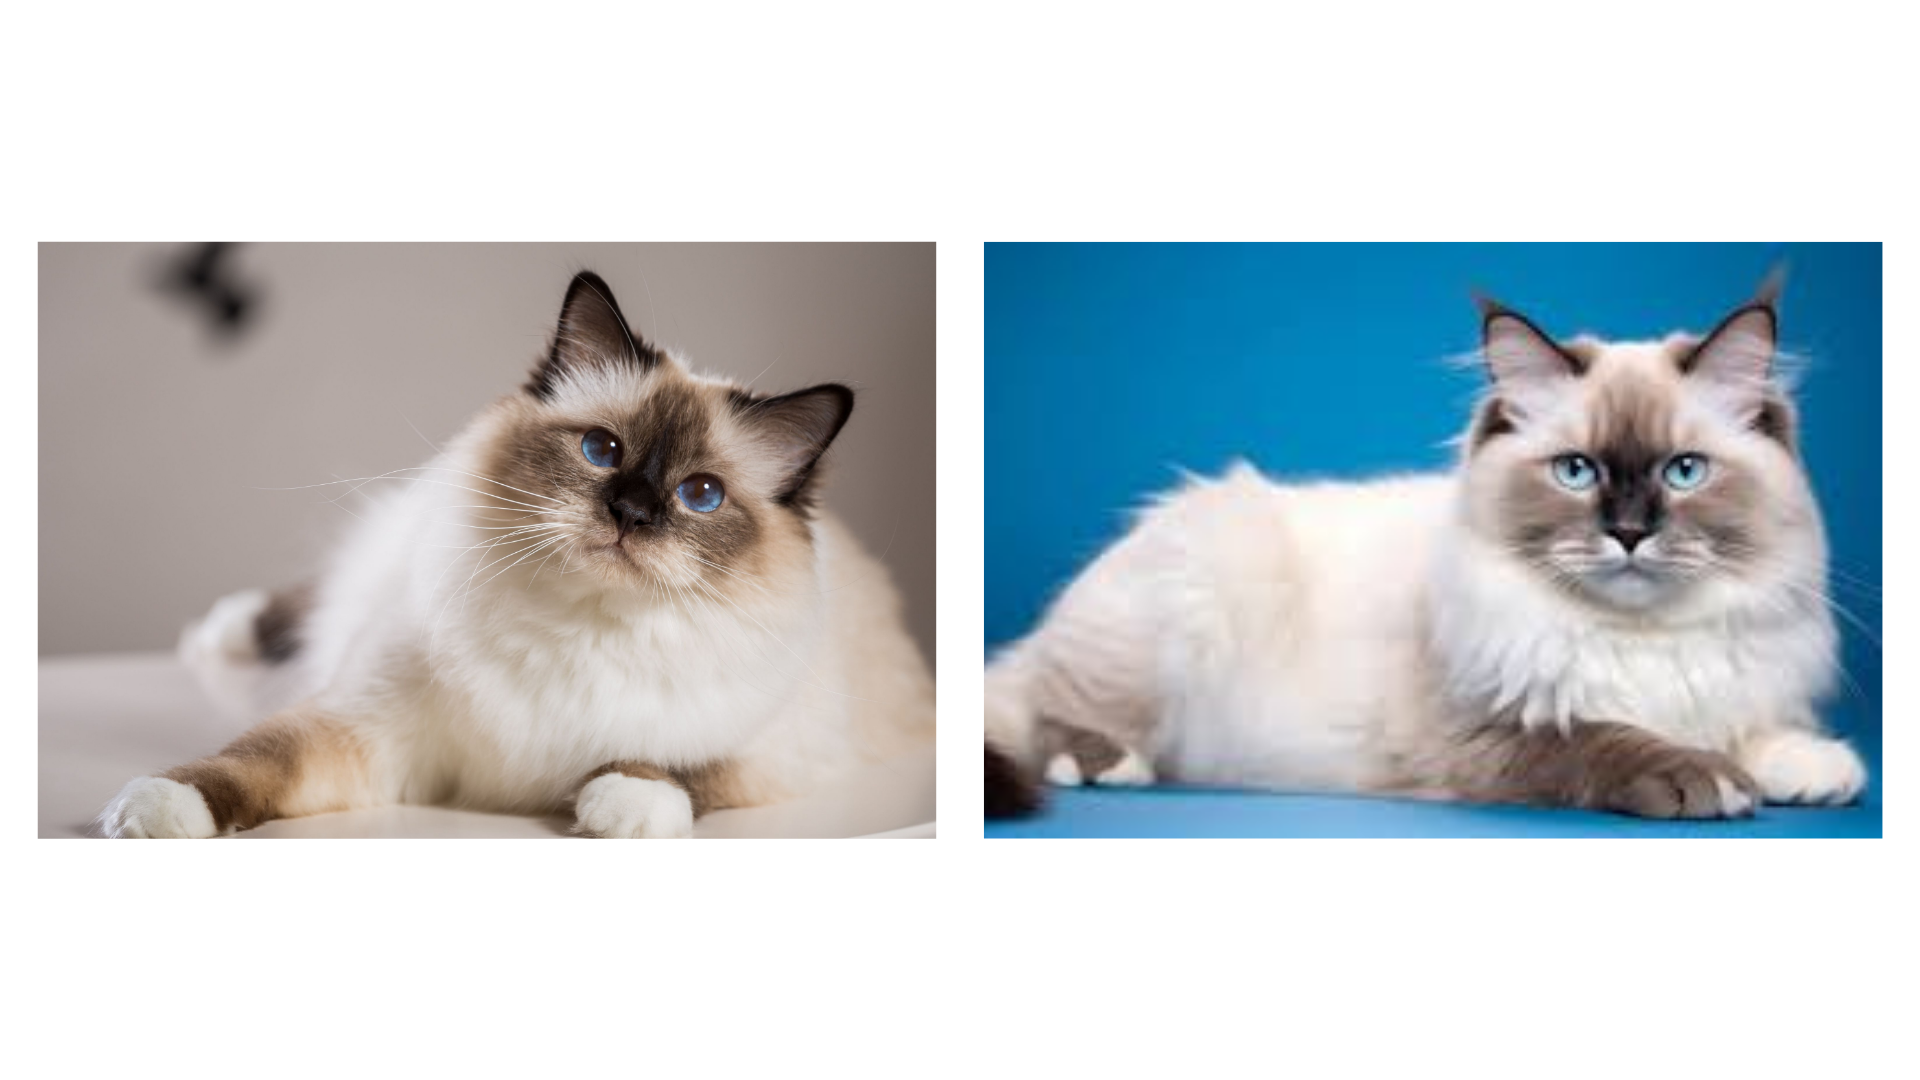
\includegraphics[width=0.7\textwidth]{figures/breed_compare.png}
    \caption{Ragdoll Cat (class no. 27) and Birman Cat (class no. 7) look almost identical}
    \label{fig:example_images}
\end{figure}
 \begin{table}[H]
    \centering
    \caption{Metric Evaluation for Complex Model}
    \begin{tabular}{|c|c|c|c|}
        \hline
        Metric & Precision & Recall & F1-score \\ 
        \hline
        Macro Average & 0.94 & 0.95 & 0.945 \\ 
        \hline
        Weighted Average & 0.96 & 0.955 & 0.955 \\ 
        \hline
    \end{tabular}
    \label{tab:complex_model_metrics}
\end{table}

\section{Comparison}
From the results of the two tables (table II and table I), it can be concluded that the use of transfer learning techniques employed in the more complex model lead to better results in all measures when compared to the simple model, even after choosing the best hyper-parameters. The difference between both of them is giant with the first one barely managing to classify an image correctly (average accuracy = 0.066), and the other doing that almost every time (average accuracy = 0.955).
\section{Summary}
In this chapter, I evaluated the simple and complex neural network models using a stratified test set and key performance metrics. The simple model struggled with classification accuracy, consistently favoring a few specific breeds, as reflected in its confusion matrix and low metric scores. In contrast, the complex model, utilizing transfer learning, performed significantly better across all metrics, demonstrating the effectiveness of this approach. This evaluation confirms that transfer learning substantially improves the model's ability to generalize and accurately classify images.